\section{Rewrite Rules}

This section introduces the various rewrite rules that come equipped with the ZX calculus. These rules extend the ZX calculus from notation into a language.

\subsection{Spider Fusion}
The most fundamental rule of the ZX calculus is the \textit{spider fusion} rule \cite{Wetering2020}. It states that two spiders connected by one or more wires fuse if they are the same colour. It is the generalisation of adding the phases of successive rotations of the Bloch sphere. Since we interpret the phases $\alpha$ and $\beta$ as $e^{i\alpha}$ and $e^{i\beta}$, it follows that the phase $\alpha + \beta$ is modulo $2\pi$.

\begin{figure}[H]
    \centering
    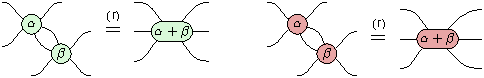
\includegraphics[width=0.8\textwidth]{chapter-2/fusion}
    \caption{Spider fusion rule for $Z$ spiders (left) and $X$ spiders (right).}
\end{figure}

Using this rule we can identify useful commutation relations. $Z$ rotations commute through CNOT controls and $X$ rotations commute through CNOT targets.
\begin{center}
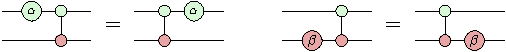
\includegraphics[width=0.9\textwidth]{chapter-2/cnot_commutation}
\end{center}

%%%

\subsection{Identity Removal}
The \textit{identity removal} rule states that any two-legged spider with no phase ($\alpha = 0$) is equivalent to an empty wire since a rotation by 0 radians is the same as no rotation.
\begin{figure}[H]
    \centering
    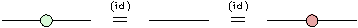
\includegraphics[width=0.7\textwidth]{chapter-2/identity}
    \caption{Identity removal rule.}
\end{figure}

Combining this with the spider fusion rule, we see that two successive rotations with opposite phases is equivalent to an empty wire.
\begin{center}
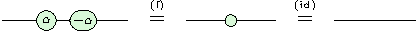
\includegraphics[width=0.8\textwidth]{chapter-2/cancelling_rotations}
\end{center}

%%%

\subsection{Bialgebra Rule}
Unlike the previous rules we have introduced, the \textit{bialgebra rule} takes some time to understand intuitively. It is nethertheless important in many derivations.
\begin{figure}[H]
    \centering
    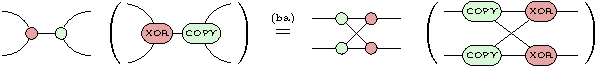
\includegraphics[width=0.5\textwidth]{chapter-2/bialgebra}
    \caption{Bialgebra rule.}
\end{figure}

We assume that the left part of the bialgebra rule (three-legged $X$ spider) behaves like the classical XOR gate with the computational basis states whilst the right part (three-legged $Z$ spider) behaves like the classical COPY gate. The latter is known as the $\pi$ copy rule (see appendix).

By considering the natural commutation relation of the classical XOR and COPY gates as motivation, it is clear that XORing the bits then copying them is indeed the same as copying then XORing.
\begin{center}
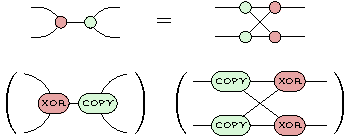
\includegraphics[width=0.6\textwidth]{chapter-2/xor_copy_zx}
\end{center}

